% !TEX root=/home/tavant/these/manuscript/src/manuscript.tex

\section{PIC simulation results of the Axial-azimuthal simulations}
  \label{sec-Zthetaresults}
  In this sections, we present the results of the \ac{2D} \ac{PIC} simulations using the test-case of Boeuf, described in \cref{subsec-boeuf_description}; the parameters used are given in \vref{tab-parameters-boeuf}.
  In this test-case, the ionization is fixed, hence the breathing mode is absent.
  Consequently, the simulation converges quickly toward a steady state.
  
  We uses the test-case of Boeuf for three different cases.
  The first is the usual case, without the effects of the radial direction.
  It is expected to return the same results as obtained in \citet{boeuf2018}.
  The two other cases model the effect of the radial direction.
  Two values of the radial length are used\string: $L_R=4\,\centi\meter$ and $2\,\centi\meter$.

  
  \subsection{Simulation results\string: an overview} \label{subsec-boeuf-overview}
  As the ionization is not self-consistently modeled, the simulations converges under $10\,\micro\second$.
  \Cref{fig-overview_boeuf_neEx} shows the axial and azimuthal distribution of the azimuthal electric field $E_{\theta}$ and the electron density $n_e$ at $t=8\,\micro\second$ is the case where no radial losses are modeled.
  We see in both $E_{\theta}$ and $n_e$ the \ac{ECDI}, which wavelength is approximately $\lambda_{\theta} = 0.08\,\centi\meter$.
  The results observed are similar to the one presented by \citet{boeuf2018}, hence we believe that there is no error in the simulation and we expect to obtain the same results.

  \begin{figure}[hbt]
    \centering
    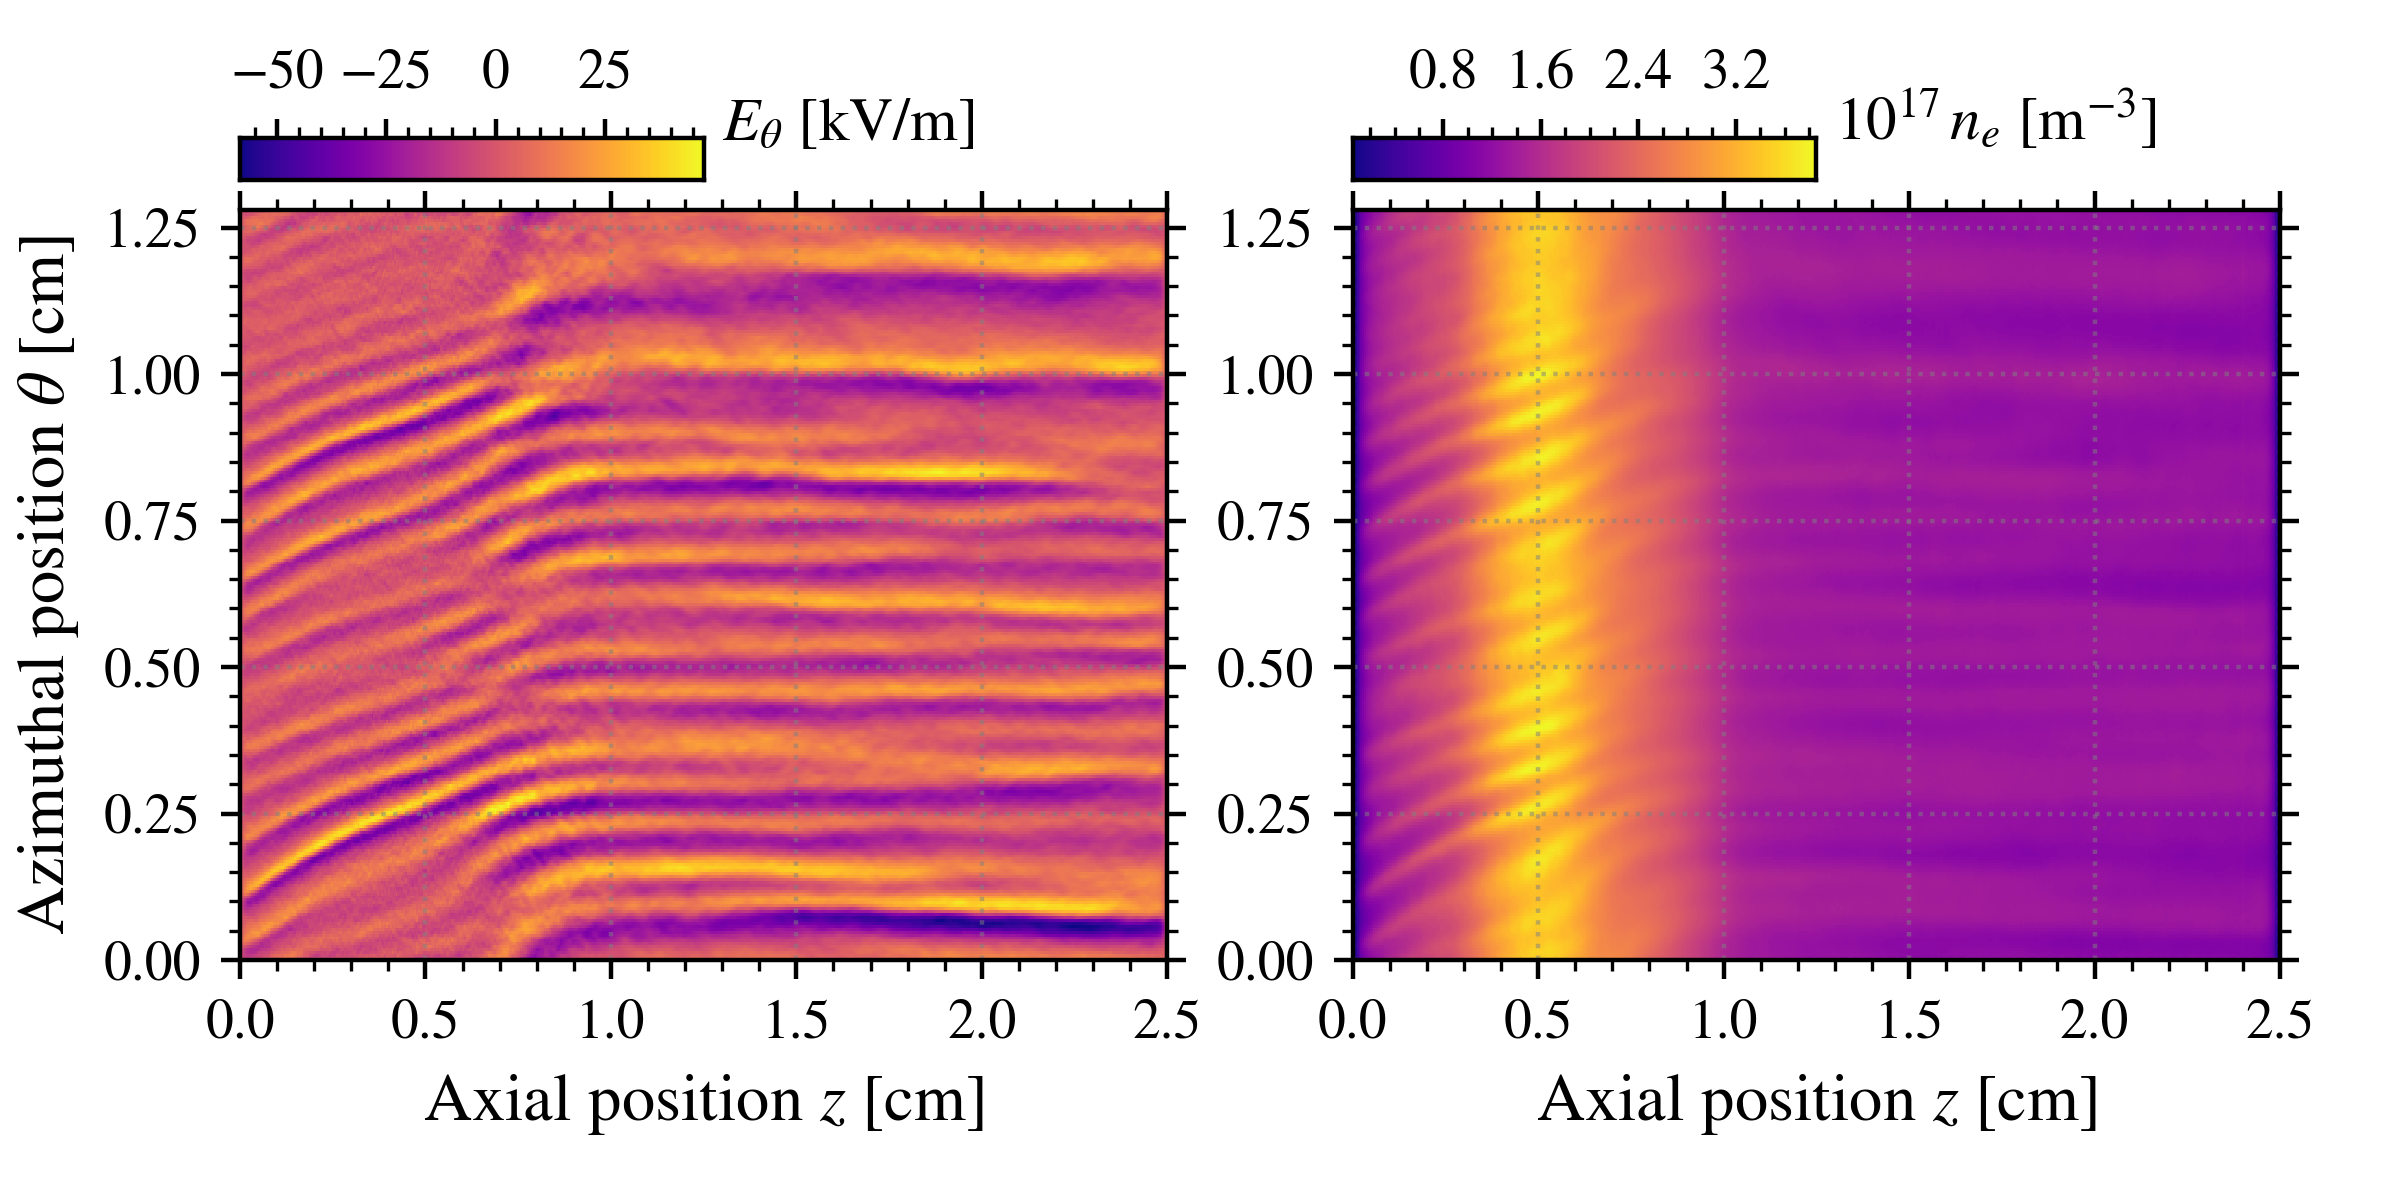
\includegraphics[width=0.9\textwidth]{Boeuf_example_t=8}
    \caption{ Axial-azimuthal distributions of (left) the azimuthal electric field $E_{\theta}$ and (right) the electron density $n_e$ at $t=8\,\micro\second$ for the test-case of Boeuf. } 
    \label{fig-overview_boeuf_neEx}
  \end{figure}

  \subsection{Simulation results\string: temporal evolution} \label{subsec-temp_boeuf}
  
  \Cref{fig-boeuf-temporal} presents the temporal evolution of the mean plasma density and temperature.
  We see that when the radial direction is modeled, the density and the mean electron temperature and the radial electron temperature is reduced, as expected when increasing the losses when the ionization source term is not self-consistent.

  \begin{figure}[hbt]
    \centering
    \begin{tabular}{cc}
      \subfigure{Boeuf_ne_temporal}{a}{20,20} &
      \subfigure{Boeuf_Te_temporal}{b}{20,20} \\
    \end{tabular}
    \caption{Temporal evolution of ({\bf a})  the mean plasma density, and  ({\bf b}) the  mean electron temperatures in the axial-azimuthal simulations, obtained with three different radial models. }
    \label{fig-boeuf-temporal}
  \end{figure}

  We see on \cref{fig-boeuf-temporal}.{\bf b} that the radial temperature remains constant when the radial direction is not modeled.
  This is due to the fact that the collisions are not modeled in the simulations, so that there is not momentum and energy transfer possible from the axial and azimuthal directions, and the radial direction.

  However, we know from the radial-azimuthal simulations that there is a transfer of energy between the axial direction and the radial direction, resulting in a plasma less anisotropic than observed here.
  This aspect is discussed latter in \cref{subsec-MCC_boeuf,subsec-radial-heating}.
  With the radial losses, the radial temperature decreases from the initial temperature $\Te=5\,\volt$ to $\Te_R\simeq 2.2$ and $ 3.3\,\volt$ for $L_R=2$ and $3\,\centi\meter$, respectively.
  The total temperature $\Te$ shows a similar decrease with the increase of the radial losses.

  \subsection{Simulation results\string: averaged axial profiles} \label{subsec-axial_boeuf}

  \Cref{fig-boeuf_axialone,fig-boeuf_axialtwo}  show the axial profile at steady-state of several plasma quantities.
  The variables are averaged in the azimuthal direction and in time during the steady-state between $t=8$ and $t=10\,\micro\second$.
  The results  obtained with three different radial models are overlaid.
  \cref{fig-boeuf_axialone}.{\bf a} shows the axial electric field $E_z$.
  The differences in $E_z$ are small, but we can still distinguish that the amplitude of $E_z$ is reduced with the increased radial losses.
  The electron density $n_e$ shown in \cref{fig-boeuf_axialone}.{\bf b} is almost not affected, except in for $z>1\,\centi\meter$, where the electron losses at the wall can be seen.

  \begin{figure}[hbt]
    \centering
    \begin{tabular}{cc}
      \subfigure{Boeuf_electric_field}{a}{30,22} &
      \subfigure{Boeuf_ne_axial}{b}{30,24} \\
    \end{tabular}
    \caption{Averaged axial profiles at steady state of ({\bf a}) the axial electric field $E_z$, ({\bf b}) the mean plasma density obtained with three different radial models for the simulation case of Boeuf. }
    \label{fig-boeuf_axialone}
  \end{figure}

  \Cref{fig-boeuf_axialtwo} shows the axial profiles of the electron axial density current and the electron temperatures.
  In contrast to $n_e$ and $E_z$, the electron temperatures are reduced by the radial losses in each direction ($\Te{}_{,\theta}, \Te{}_{,R}, \Te{}_{,Z}$).
  The radial temperature $\Te{}_{,R}$ is reduced uniformly everywhere, but the two other temperature are mostly affected before the axial position of their maxima, at approximately $z=0.8$.
  However, the radial losses should not reduce the axial and azimuthal temperatures.
  The electron heating comes principally from the Joule heating $\vect{J_e} \cdot \vect{E}$.
  As axial electric field $E_z$, seen in \cref{fig-boeuf_axialone}.{\bf a}, is almost unaffected, the difference in the electron temperature necessaryly comes from the differences in the axial electron current.

  \begin{figure}[hbt]
    \centering
    \begin{tabular}{cc}
      \subfigure{Boeuf_Te_axial}{a}{25,80} &
      \subfigure{Boeuf_Je_axial}{b}{30,22} \\
    \end{tabular}
    \caption{Averaged axial profile at steady state of ({\bf a}) the  electron temperature, and ({\bf b}) the axial electron current density $J_{e, z}$, obtained with three different radial models for the simulation case of Boeuf. }
    \label{fig-boeuf_axialtwo}
  \end{figure}
  
  The axial electron density current $J_{e, z}$ \cref{fig-boeuf_axialtwo}.{\bf b} is even more significantly reduced by the radial losses.
  We observe a factor of two on $J_{e, z}$ between the case $L_R=2\,\centi\meter$ and the case without losses.
  As we have seen in \cref{fig-boeuf_axialone}.{\bf b} that the electron density is almost unaffected.
  This means that the electron axial velocity is reduced by the radial losses.
  \Cref{fig-mobility} shows the average axial mobility \[ \mu_e = \frac{J_e}{-e n_e E_z}  \]

  \begin{figure}[hbtp]
    \centering
    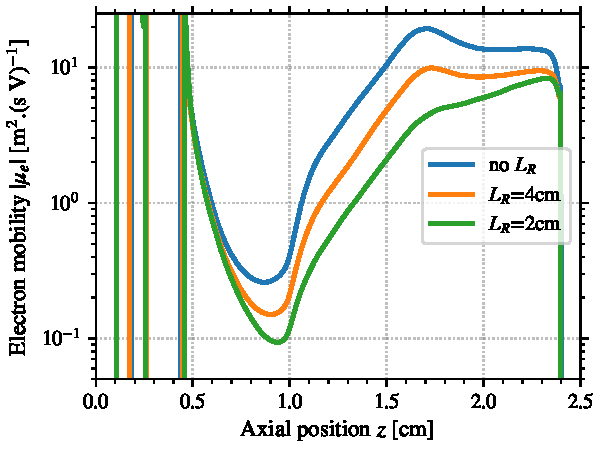
\includegraphics[width=\defaultwidth]{Boeuf_axial_mobility.pdf}
    \caption{Axial profile of the electron mobility measured in the \ac{PIC} simulations for the three cases of radial losses, in logarithmic scale.}
    \label{fig-mobility}
  \end{figure}

  We can see that the electron mobility is reduced significantly affected by the radial losses.
  However, since the the simulation is collisionless, the electron crossfield transport in the axial direction is only due to the azimuthal instability
  It is confirmed by the values presented in \Cref{fig-boeuf-instability}, that shows on the left the average standard deviation of the azimuthal electric field, and on the right the correlation term $R_{ei}$.
  We recall from \cref{sec-transport} that 
  \begin{equation} \label{eq-rei}
    R_{ei} =  - e < \dne \dEt >_{\theta},
  \end{equation}
  wuth $\dne$, and $\det$ the fluctuations of the electron density and azimuthal electric field, respectively.
  Moreover, we have from \cref{eq-mobeffsimple}
  \begin{equation*}
    \mu_e = \frac{< \dne \dEt >_{\theta} }{n_0 E_z}   \frac{1}{B_r}
  \end{equation*}


  \begin{figure}[hbt]
    \centering
    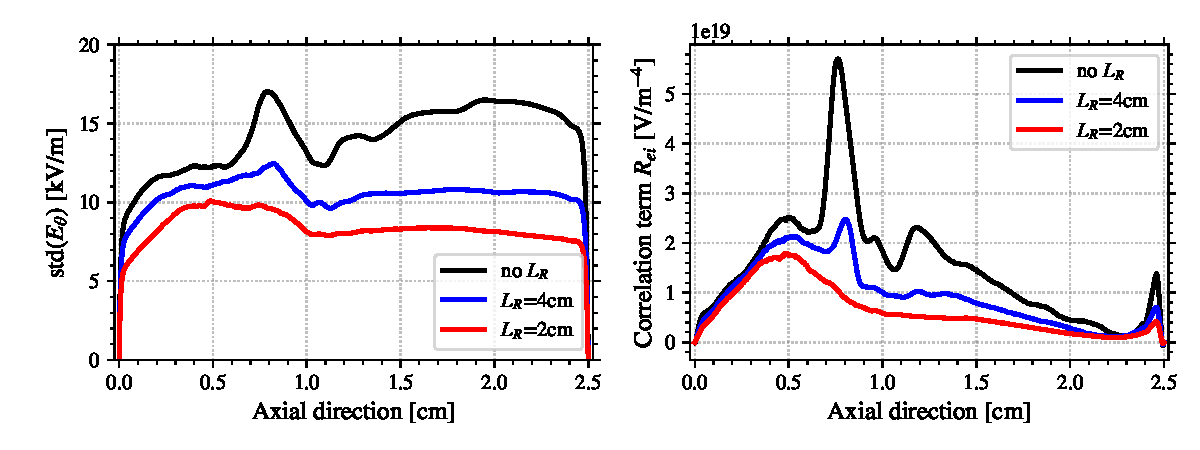
\includegraphics[width=\textwidth]{Boeuf_instability_characteristics}
    \caption{Axial profiles of the characteristics of the instability, (left) average of the standard deviation of the azimuthal electric field, (right) electron-ion friction force calculated by the correlation between $n_e$ and $\Te$.    }
    \label{fig-boeuf-instability}
  \end{figure}

  
  We observe in \cref{fig-boeuf-instability} that the amplitude of the instabilities, as well as the correlation term, are significantly affected by the electron radial losses.
  
  To summarized the results presented in this section, we used a simple model to model the radial particle losses in the axial-azimuthal simulation.
  We observe almost no impact on the axial electric field $E_z$, and a slight diminution of the mean electron density (up to 20\% in total, but mostly present in the near-plume region).
  
  The electron temperature is also reduced, not only in the radial direction, where the radial losses have a direction impact, but also on the azimuthal and axial temperatures.
  This is consistent with the large reduction of the axial electron mobility, which lower the joule heating.
  The reduction of the crossfield electron transport comes from the diminished amplitude of the azimuthal instability.
  
  Before analyzing in more details the instability in \cref{sec-Ztheta-instability}, we discuss in the next section the problematic of the radial electron heating.


  \section{Radial electron heating}
    We have seen in \cref{fig-boeuf-temporal,fig-boeuf_axialtwo} that the radial electron temperature is constant in both time and space, leading to a large anisotropy.
    This could be due to the lack of collision in the test-case of Boeuf
    Thus, we investigate thereafter the impact of the neutrals on the electron anisotropy by modeling the collisions with the \ac{MCC} algorithm.
    
  \subsection{Boeuf test-case with collisions} \label{subsec-MCC_boeuf}
  % Script on Juno (CH-6_Boeuf)

  To model the neutral density, we inject at the anode a constant xenon flow of rate $m_a = 5 \milli\gram\per\second$ at a temperature of $T_g = 640\,\kelvin$.
  Using a typical surface area, this corresponds to a neutral density at the anode of $n_g=3.0 \times 10^{19}$ {m}$^{-3}$ and a mean velocity of $u_g = 200 \,\meter\per\second$.
  
  The evolution of the neutral density is model using the system of \ac{1D} fluid equations, as we neglect the evolution in the azimuthal direction\string:
  \begin{equation}
  \left\{
  \begin{gathered}
  \partial_{t} n_g + \partial_{z}(n_g u_g) = - S_{iz}\\
  \partial_{t}(n_g u_g) + \partial_{z}(n_g u_g^{2}) = -\partial_{z}p_g - S_{iz} u_g \\
  \partial_{t}E + \partial_{z}(Eu_g) = - \partial_{z}(pu_g)
  \end{gathered}
  \right.
  \label{eq-euler}
  \end{equation}
  with $u_g, p_g$ the neutral axial velocity and the pressure, respectively, $S_{iz}$ is the imposed ionization source term, and $E$ the energy per volume unit
  \begin{equation}
    E =  \frac{p}{\gamma - 1} + \frac{1}{2} n_g u^{2},
  \end{equation}
  with $\gamma=5/3$.
  This Euler system is solved using the HLLC Riemann solver, which as been validated on the  shock tube test case.
  For sake on simplicity, the neutral temperature is kept constant by adding an artificial source term is the third equation of \cref{eq-euler}
  \begin{equation} \label{eq-artificial}
    S_3 = -\frac{1}{\tau} \lp  \frac{p}{\gamma - 1} - \frac{n_g R T_0}{\gamma-1} \rp
  \end{equation}
  with $T_0$ the desired temperature, and $\tau$ the "thermalization time" to reach the $T_0$.
  We chose $\tau$ small enough so that $T_n$ does not vary much, while preserving the Courant-Friedrich-Levy condition.
  In practice, we use $\tau = 10\,\micro\second$.
  
  Finally, the neutral density is used in the \ac{MCC} algorithm to model the electron-neutral and ion-neutral scattering and momentum transfer, but the creation of particles remains imported by same the ionization profile $S_iz$ as in \cref{sec-Zthetaresults}.
  \Cref{fig-boeuf-neutrals} shows the neutral density and velocity obtained at steady-state.

  \begin{figure}[hbt]
    \centering
    \begin{tabular}{cc}
      \subfigure{boeuf_MCC_ng}{a}{20,20} &
      \subfigure{boeuf_MCC_vg}{b}{20,15} \\
    \end{tabular}
    \caption{Axial profile at steady-state ($t=10\,\micro\second$) of ({\bf a}) the neutral density and  ({\bf b})  the neutral axial velocity, for  simulation with the electron-neutral scattering. }
    \label{fig-boeuf-neutrals}
  \end{figure}
  \inlinenote{The figure x label is wrong}

  We see in \cref{fig-boeuf-neutrals} that the neutral density is significantly depleted because of the forced ionization source term.
  The neutral density gradient accelerates the neutrals in the axial direction by a factor of two, which reduces even more the neutral density.
  Thus, the impact of the neutral collisions will be more significant on the anode side of the chamber.

  \begin{figure}[hbt]
    \centering
    \begin{tabular}{cc}
      \subfigure{boeuf_mean_Te}{a}{20,20} &
      \subfigure{boeuf_mean_Tez_profile_MCC}{b}{20,15} \\
    \end{tabular}
    \caption{({\bf a}) temporal evolution of the electron kinetic energy in the three directions and  ({\bf b}) axial profile of the electron temperature at steady state obtained for the simulation case of Boeuf with the electron-neutral scattering. }
    \label{fig-boeuf-temporalMCC}
  \end{figure}

  \Cref{fig-boeuf-temporalMCC} shows the temporal evolution of the mean electron kinetic energy on the left, and on the right it shows the axial profile of the electron temperatures, decomposed on the three directions.
  We see that they is a small transfer of energy between the radial direction and the others.
  In particular, close to the anode where the gas density is high, the radial and axial temperatures decrease below the initial temperature $\Te_{, inj}=5\,\volt$.
  In contrast, at the maximum of the magnetic field where the axial and azimuthal electron temperatures are the highest, the radial electron temperature increases to $\Te_R=7\,\volt$.
  However, the anisotropy stays significant, compared to the observation of the radial-azimuthal simulations presented in \cref{ch-2}.
  therefore, the neutral density is not the main reason for the electron heating.

  \subsection{Radial heating of electrons in the radial-azimuthal simulation} \label{subsec-radial-heating}
  
  The large anisotropy observed in \Cref{fig-boeuf-temporal,fig-boeuf-temporalMCC}, compared to the results of \cref{ch-2} does not come from the electron-neutral scattering.
  Thus in this section, we investigate the electron energy gain due to Joule heating
  \begin{equation} \label{eq-epower}
      \vect{P_{\rm J}} = \vect{J_e} \cdot \vect{E},
  \end{equation}
  with $\vect{J_e}$ the electron density current and $\vect{E}$ the electric field.
  \Cref{fig-epower_radialone} shows the radial profiles of the electron (and ion) current density $< J_{e, R}>$ and the radial electric field $ < E_R >$, averaged in the azimuthal direction.
  We observe that the ion and electron current densities are equal to each-other, and they increase linearly with the radial position.
  This was expected, as we use a uniform artificial injection of particles, which compensates the radial losses (see \cref{sec-bidimentionnal_simulation} for more details).

  \begin{figure}[hbt]
    \centering
    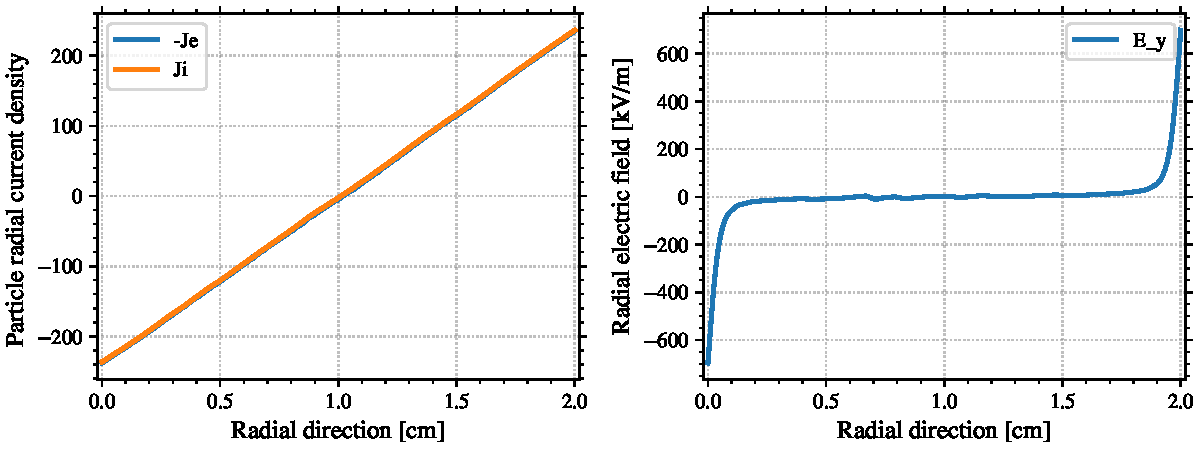
\includegraphics[width=\textwidth]{R_joule_heating_one}
    \caption{Radial profiles averaged in the azimuthal direction of (left) the electron and ion current densities and (right) radial electric field in the radial-azimuthal \ac{PIC} simulation presented in \cref{ch-2}. }
    \label{fig-epower_radialone}
  \end{figure}
  \inlinenote{Wrong legends : $E_y$, and put $J_e$ in A/m$^2$.}
  
  The radial electric field $E_r$ seen in \cref{fig-epower_radialone} is very small in the center of the system, and increases drastically in the sheath close to the walls.
  Consequently, from the product $< J_{e, R}>  < E_R >$ we could expect that the radial Joule electron heating to be small in the center of the discharge, and negative in the sheath.

  \Cref{fig-epower_radial} shows the mean Joule heating in the radial direction $\bar{P_{\rm J, R}} = < J_{e, R} E_R >$ measured in the \ac{PIC} radial-azimuthal simulation, and the product of the mean quantities $< J_{e, R}>  < E_R >$.

  \begin{figure}[hbt]
    \centering
    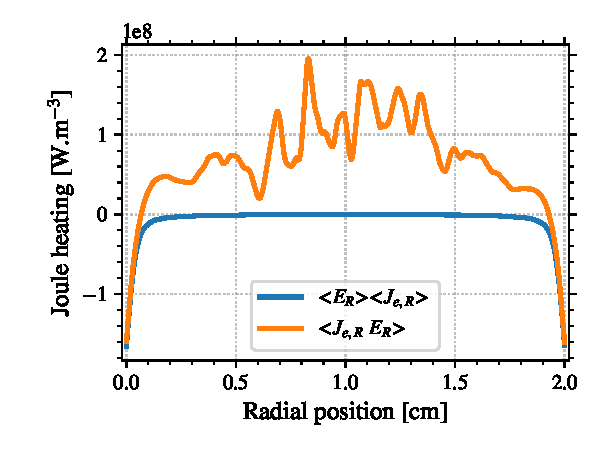
\includegraphics[width=\defaultwidth]{R_joule_heating_two}
    \caption{Electron power gain in the Radial-azimuthal }
    \label{fig-epower_radial}
  \end{figure}

  We see in \Cref{fig-epower_radial} that, unexpectedly,  the mean Joule heating $\bar{P_{\rm J, R}}$ is not zero in the center of the simulation.
  This means that there is an energy transfer to the radial direction of the electrons due to the correlation between the fluctuations of $\vect{J_e}$ and $\vect{E}$.
  Consequently, for this energy transfer to be self-consistently observe, the radial direction needs to be resolved.

  A similar radial heating has been observed by \citet{heron2013}.
  The authors observe no heating when the instability was only perpendicular to the magnetic field, as it is in a \ac{1D} or a \ac{2D} axial-azimuthal simulation.
  However, when the direction parallel to the magnetic field is resolved, the electrons are heated.
  However, but the physical mechanism remains unclear.
  In \citet{janhunen}, the authors observe a similar radial heating of the electrons, but due to the presence of a \ac{MTSI}.
  As discussed in the previous chapters, we do not observe the \ac{MTSI} in our simulations, meaning that it has to be due to another mechanism.


